\documentclass[]{article}
\usepackage{lmodern}
\usepackage{amssymb,amsmath}
\usepackage{ifxetex,ifluatex}
\usepackage{fixltx2e} % provides \textsubscript
\ifnum 0\ifxetex 1\fi\ifluatex 1\fi=0 % if pdftex
  \usepackage[T1]{fontenc}
  \usepackage[utf8]{inputenc}
\else % if luatex or xelatex
  \ifxetex
    \usepackage{mathspec}
  \else
    \usepackage{fontspec}
  \fi
  \defaultfontfeatures{Ligatures=TeX,Scale=MatchLowercase}
\fi
% use upquote if available, for straight quotes in verbatim environments
\IfFileExists{upquote.sty}{\usepackage{upquote}}{}
% use microtype if available
\IfFileExists{microtype.sty}{%
\usepackage{microtype}
\UseMicrotypeSet[protrusion]{basicmath} % disable protrusion for tt fonts
}{}
\usepackage[margin=1in]{geometry}
\usepackage[unicode=true]{hyperref}
\hypersetup{
            pdftitle={working owls methods},
            pdfauthor={Althea Archer},
            pdfborder={0 0 0},
            breaklinks=true}
\urlstyle{same}  % don't use monospace font for urls
\usepackage{graphicx,grffile}
\makeatletter
\def\maxwidth{\ifdim\Gin@nat@width>\linewidth\linewidth\else\Gin@nat@width\fi}
\def\maxheight{\ifdim\Gin@nat@height>\textheight\textheight\else\Gin@nat@height\fi}
\makeatother
% Scale images if necessary, so that they will not overflow the page
% margins by default, and it is still possible to overwrite the defaults
% using explicit options in \includegraphics[width, height, ...]{}
\setkeys{Gin}{width=\maxwidth,height=\maxheight,keepaspectratio}
\IfFileExists{parskip.sty}{%
\usepackage{parskip}
}{% else
\setlength{\parindent}{0pt}
\setlength{\parskip}{6pt plus 2pt minus 1pt}
}
\setlength{\emergencystretch}{3em}  % prevent overfull lines
\providecommand{\tightlist}{%
  \setlength{\itemsep}{0pt}\setlength{\parskip}{0pt}}
\setcounter{secnumdepth}{0}
% Redefines (sub)paragraphs to behave more like sections
\ifx\paragraph\undefined\else
\let\oldparagraph\paragraph
\renewcommand{\paragraph}[1]{\oldparagraph{#1}\mbox{}}
\fi
\ifx\subparagraph\undefined\else
\let\oldsubparagraph\subparagraph
\renewcommand{\subparagraph}[1]{\oldsubparagraph{#1}\mbox{}}
\fi

\title{working owls methods}
\author{Althea Archer}
\date{11/3/2020}

\begin{document}
\maketitle

\section{Methods}\label{methods}

\subsection{Occupancy Model}\label{occupancy-model}

Let

\[
\begin{aligned}
t  &=  \text{the years of surveys (here }t = 1,2,\ldots,11)\\
h  &=  \text{the individual routes (here }h = 1,2,\ldots,6)\\
i  &=  \text{the individual surveys conducted in each year and route (here }i = 1,2,3)\\
j  &=  \text{the individual stations along each route (here }j = 1,2,\ldots,10)\\
k  &=  \text{the broadcast species (here }k = 1,2,\ldots,10)\\
z_{t,h,i} &= \text{a random variable equal to 1 when a survey was occupied and 0 otherwise}\\
y_{t,h,i,j,k} &= \text{a random variable equal to 1 when an owl was detected and 0 otherwise}
\end{aligned}
\]

We assumed that survey occupancy (\(z_{t,h,i}\)) was the outcome of
Bernoulli trials with probability \(\psi\), which we allowed to vary by
year and route:

\[
z_{t,h,i} \sim \text{Bernoulli}(\psi_{t,h})
\]

\[
\psi_{t,h} \sim \text{Beta}(a^\psi_{t,h},b^\psi_{t,h})
\] with hyperpriors for \(a^\psi_{t,h}\) and \(b^\psi_{t,h}\) such that
the expected value of \(\psi_{t,h} = \mu^\psi_{t,h}\):

\[
\begin{aligned}
\text{E}[\psi_{t,h}] &= \mu^\psi_{t,h} = a^\psi_{t,h}/(a^\psi_{t,h}+b^\psi_{t,h})\\
\rho^\psi_{t,h} &= a^\psi_{t,h}+b^\psi_{t,h}\\
\mu^\psi_{t,h} &\sim \text{Uniform}(0.01, 0.99)\\
\rho^\psi_{t,h} &\sim \text{N}(5,1)\text{, truncated to 0.01,10}\\
\end{aligned}
\]

We assumed that detecting an owl depended on an owl being present during
that survey (\(z_{t,h,i} = 1\)) and the probability of detection, which
was related to the broadcast species:

\[
y_{t,h,i,j,k} \sim \text{Bernoulli}(z_{t,h,i}*p_{t,h,i,j,k})
\]

where generally \(\text{logit}(p_{t,h,i,j,k}) = \beta_kX_k\), or more
specifically:

\[
\begin{aligned}
\text{logit}(p_{t,h,i,j,k}) &= \beta_\text{Pre-broadcast}X_\text{Pre-broadcast} + \\
&= \beta_\text{Mottled}X_\text{Mottled}+\\
&= \beta_\text{Pacific}X_\text{Pacific}+\\
&= \beta_\text{Crested}X_\text{Crested}+\\
&= \beta_\text{Black and White}X_\text{Black and White}+\\
&= \beta_\text{Spectacled}X_\text{Spectacled}+\\
&= \beta_\text{Whiskered}X_\text{Whiskered}+\\
&= \beta_\text{Guat Barred}X_\text{Guat Barred}+\\
&= \beta_\text{Stygian}X_\text{Stygian}+\\
&= \beta_\text{Great Horned}X_\text{Great Horned}\\
\end{aligned}
\]

This model provides a consistent probability of detection for all
surveys in the first two minutes of each survey before the broadcast owl
recording was played. Then, the probability of detection for each
post-broadcast time period would depend on the species of broadcast owl.
This allowed species-specific behavior in response to the different
broadcast owl species (Baumgardt et al. 2019). We used means
parameterization such that the coefficients were interpretable as the
effect of that specific broadcast species \(k\) (including the
pre-broadcast time frame). The broadcast species were consistent at each
station across years, but varied by route:

\begin{table}[]
\centering
\caption{Transformations Associated with the Johnson System}
\begin{tabular}{|l|l|l|l|}
\hline
Johnson Family & Transformation & Parameter Conditions & X Condition \\ \hline
$S_B$ & $Z=\gamma + \eta ln(\frac {X - \epsilon} {\lambda + \epsilon - X})$ & $\eta, \lambda >0, -\infty < \gamma, \epsilon < \infty$ & $\epsilon < X < \epsilon + \lambda$ \\ \hline
$S_L$ & $Z=\gamma + \eta ln(X - \epsilon)$ & $\eta >0, -\infty < \gamma, \epsilon < \infty$ & $X > \epsilon$ \\ \hline
$S_U$ & $Z=\gamma + \eta \sinh^{-1}(\frac {X - \epsilon} {\lambda})$ & $\eta, \lambda >0, -\infty < \gamma, \epsilon < \infty$ & $-\infty < X < \infty$ \\ \hline
\end{tabular}
\end{table}

The priors for every logistic model coefficient \(\beta_k\) were chosen
to be near uniform as recommended in Gelman et al. (2008). Specifically,
we used the Cauchy prior as such:
\(\beta_k \sim \text{Cauchy}(\text{precision} = 0.16)\).

\subsubsection{Implementation of Occupany
Model}\label{implementation-of-occupany-model}

We used the R2jags package in R (R Development Core Team 2014,Plummer
(2013)) to implement the occupancy model for three owl species: Mottled,
Spectacled, and FerPy owls. These owls had enough positive detections to
analyze occupancy, as Mottled, Spectacled, and FerPy owls had 542, 137,
and 187 positive detections over the 11 year period, respectively. Based
on our understanding of owl ecology, we assumed that Spectacled and
FerPy owls would not occupy route M1 in Montecristo, so we removed that
route from those occupancy models.

For all three species' occupancy models, we ran 3 chains for 10,000
iterations and 1000 iterations discarded as burn-in, for a total of
27,000 iterations comprising the posterior distributions for each model
parameter. We visually inspected traceplots to verify that chains mixed
well (Supplemental information S1-3xx).

\section{Results}\label{results}

\subsection{Results sub-section}\label{results-sub-section}

\section{Discussion}\label{discussion}

You can cite references using the \textbf{citr} add-in. With
\textbf{citr} you can cite papers in line like ({\textbf{???}}) is fond
of doing, or parenthetically (R Development Core Team 2014). You can
also cite multiple sources at once ({\textbf{???}}, {\textbf{???}},
Plummer 2013). References can be added into the myrefs.bib file
directly, or created with BibTeX through LaTeX.

\section{Figures}\label{figures}

Figures can be included with the following code, but they must be in
.png format to show up in both Word and PDF. They can be referenced for
the PDF with Fig. \ref{figure1}. \emph{Unfortunately, I don't yet know
how to make the reference number show up in Word.}

\begin{figure}[htbp]
\centering
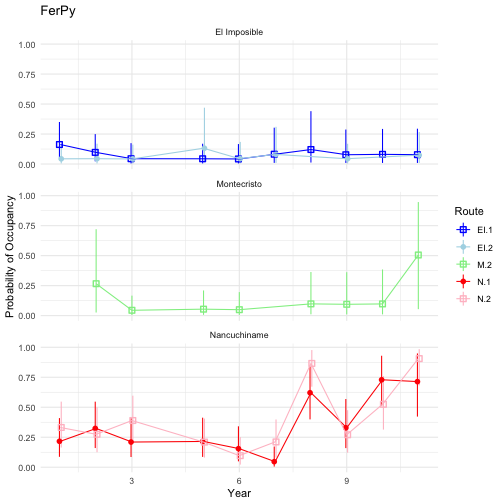
\includegraphics{../output/figures/ferpy_psi_byYr-1.png}
\caption{1. Example figure caption, which can include in-line equations
like \(y = \alpha + \beta x\) and references like ({\textbf{???}}).
\label{figure1}}
\end{figure}

\section*{References}\label{references}
\addcontentsline{toc}{section}{References}

\hypertarget{refs}{}
\hypertarget{ref-Baumgardt:2019}{}
Baumgardt, J. A., M. L. Morrison, L. A. Brennan, and T. A. Campbell.
2019. Effects of broadcasting calls on detection probability in
occupancy analyses of multiple raptor species. Western North American
Naturalist 79:185--194.

\hypertarget{ref-Gelman:2008}{}
Gelman, A., A. Jakulin, M. G. Pittau, and Y.-S. Su. 2008. A weakly
informative default prior distribution for logistic and other regression
models. The Annals of Applied Statistics 2:1360--1383.

\hypertarget{ref-Plummer:2013}{}
Plummer, M. 2013. JAGS Version 3.4.0 user manual.

\hypertarget{ref-R:2014}{}
R Development Core Team. 2014. R: A Language and Environment for
Statistical Computing. R Foundation for Statistical Computing, Vienna,
Austria.

\end{document}
